% -*- TeX-master: "../dipole_ilya_paper.tex" -*-
\section{Characterisation}
\label{sec:characterisation}
The energy spectrum of Fig.~\ref{fig:experiment} is taken on the qubit whose transitions energies fell within the 1-40\,GHz
frequency range of our microwave setup. An external magnetic field is applied perpendicular to the plane of the qubit, linking
fluxes $ \Phi = \frac{\varphi}{2\pi}\Phi_0$ and $ \eta\Phi $ ($ \eta $ is the area asymmetry of the two loops). The
\iket{1}$\,\rightarrow\,$\iket{2} transition (blue) is mapped by sweeping microwave signals and probing their tranmission on a Vector
Network Analyzer (VNA). The \iket{2}$\,\rightarrow\,$\iket{3} transition (red) is mapped using two-tone spectroscopy: a VNA is dynamically
tuned to probe frequency $ \omega_{21} $, populating state \iket{2}, while an additional microwave generator sweeps a second frequency,
$ \omega $. Whenever $\omega$ strikes the \iket{2}$ \,\rightarrow\,$\iket{3} transition ($\omega = \omega_{32} $), the qubit will be excited in sequence
\iket{1} \ira \iket{2} \ira \iket{3} and continue to be driven between states \iket{2} \iket{3}. This depopulates state \iket{1}
and the VNA probe, $ \omega_{21} $, passes with a high transmission. Thus we extract the energy profile of the system as a function of
the magnetic


\begin{figure}[h]
  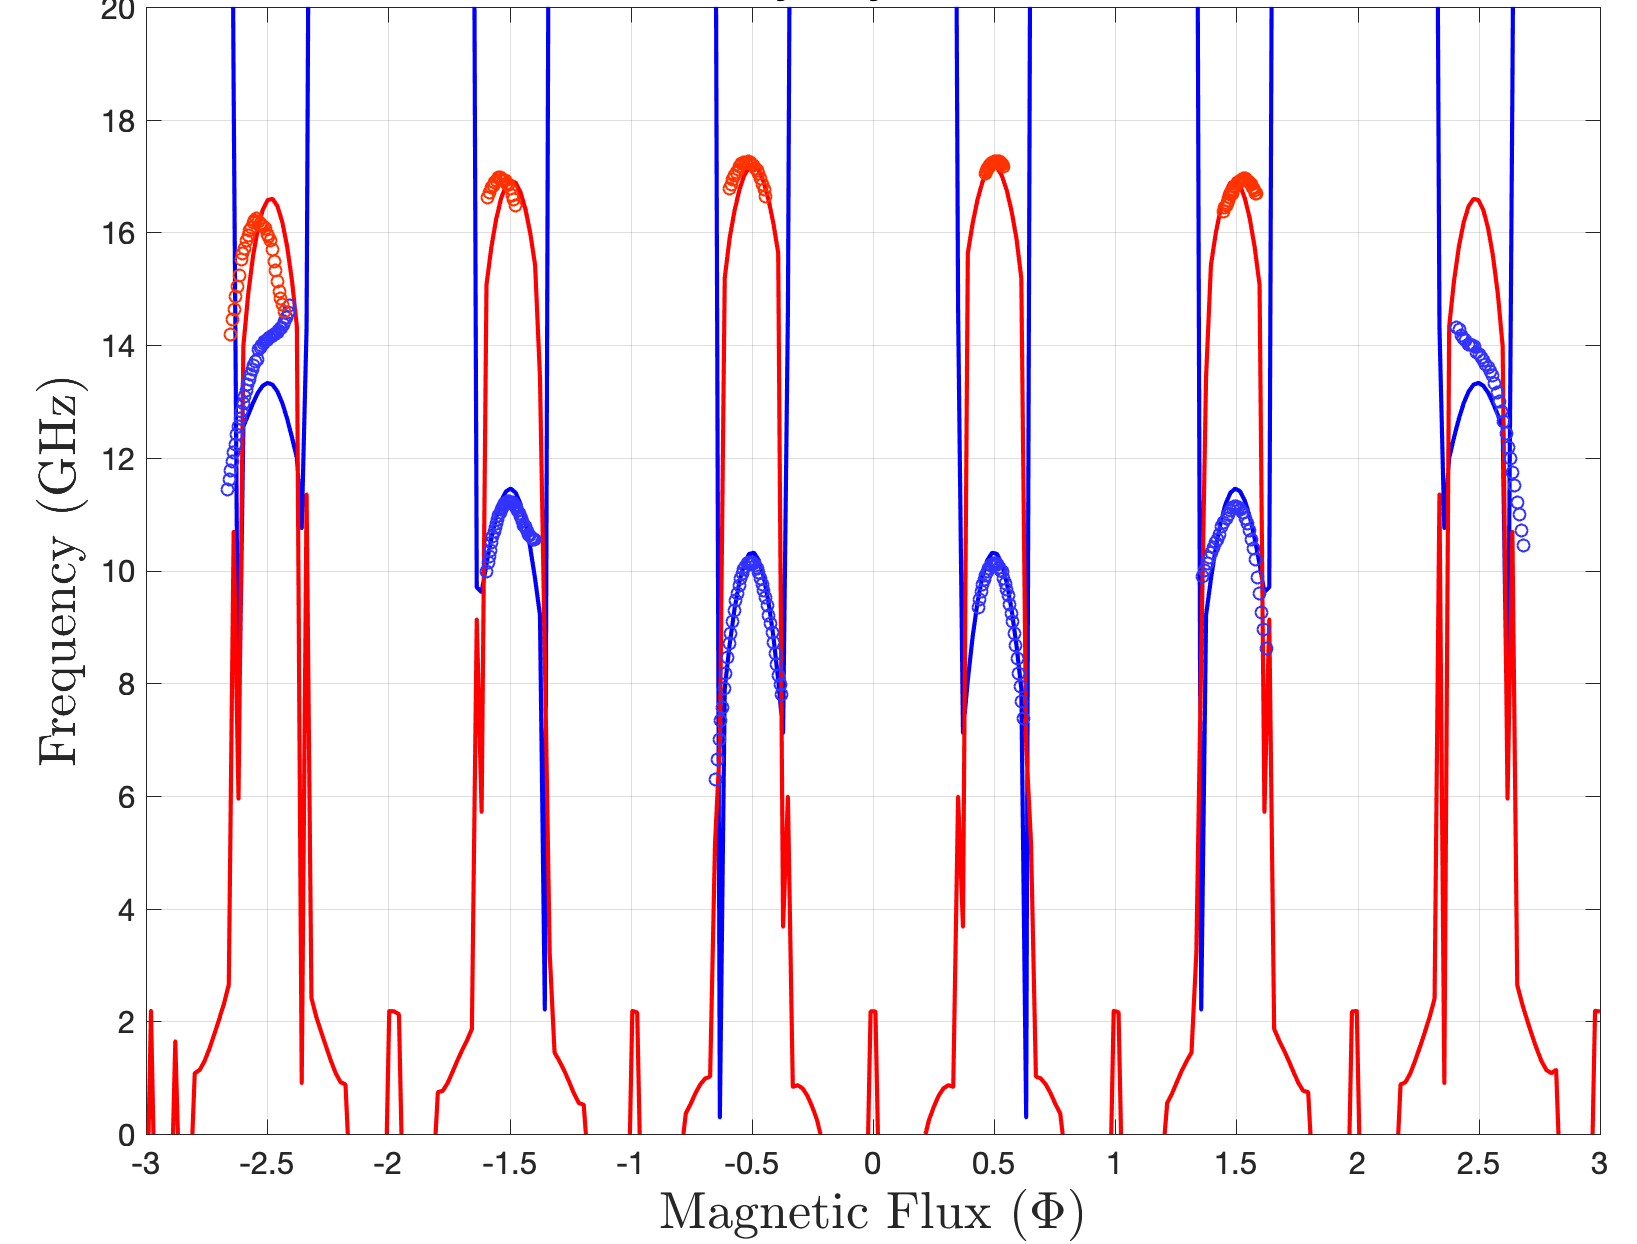
\includegraphics[height=5.5cm]{figure3_qubit2}
  \caption{\small Transition frequencies on the twin qubit between the lowest lying levels, $ \omega_{21} $ (blue) and
    $ \omega_{32}$ (red). Assymetry in the flux penetrating the left and right loops results in their gradual offset and rise away from
    $ \Phi = 0 $, breaking the usual $ \Phi_0 $ periodicity of flux systems. Readings for $ \omega_{32} $ are abrupt because with each step
    from $ \Phi = (n + \frac{1}{2})\Phi_0, n\in\mathbb{Z} $, it gets harder to tune the VNA to $ \omega_{21} $ (as part of the two-tone
    spectroscopy procedure) which prevents the further mapping of $ \omega_{32} $ with the second tone.}
  \label{fig:experiment}
\end{figure}

\noindent We match the experimental data points to simulations on the system's Hamiltonian, $ \mathcal{H} = T + V $:
\begin{itemize}
	
\item The kinetic term arises from the electrostatic charging energy of the Cooper pairs on the capacitive elements of the JJ's:
	
  \begin{equation}\label{eq:kinetic}
    \begin{aligned}
      T & = \sum_{i>j}\frac{Q_iQ_j}{2C_{ij}} = \frac{(2e)^2}{2}n\hat{C}^{-1}n^{T}.
    \end{aligned}
  \end{equation}
	
  \noindent Capacitance matrix
  $ C=\iabs{C}\left(\begin{smallmatrix} 2 & -1 & 0\\ -1 & 2 + \alpha & -1\\
      0 & -1 & 2 \end{smallmatrix}\right)$ is derived from the topology of the system in Fig.~\ref{fig:setup}. \iabs{C} is the
  capacitance of the outer JJ's.  $ \vec{n} = (n_1, n_2, n_3) $ is the number of Cooper pairs on each of the non-grounded islands.
	
\item The contribution of the 5 JJs to the potential term $ U $:
  \begin{equation}\label{eq:potential}
    \begin{aligned}
      U & = E_J\big[4 + \alpha - \alpha\cos(\varphi_{2}) -\cos(\varphi_{1}) -\cos(\varphi_{3}) - \\ & \qquad \cos(\varphi_{2} - \varphi_{1} - \varphi_{\text{ext}}) - \cos(\varphi_{2} -
      \varphi_{3} + \eta\varphi_{\text{ext}})\big].
    \end{aligned}
  \end{equation}
	
  \noindent The external fluxes are expressed in the form of phases $ \varphi_\text{ext} $, $ \eta\varphi_\text{ext} $ define phases across three
  of the JJs, $ \vec{\varphi} = (\varphi_1, \varphi_2, \varphi_3) $. All other phases in the system are pinned from the requirement of flux quantisation,
  $ \sum_i^{\text{loop}} \varphi_i = 2\pi n $.
\end{itemize}

\noindent The Hamiltonian matrix is encoded in the charge-basis, $\vec{n} $, in which the kinetic terms align on the diagonal axis
and the potential terms are distributed symmetrically on the off diagonal positions (phase operators reads
$ e^{\pm i\hat{\varphi}_j} = \sum_{n_i}\ketbra{n_i\pm1}{n_i}$ \cite{phase}). Experimental data of Fig.~\ref{fig:experiment} is fitted by
taking the eigenenergies with \iunit{E_J = 91.0}{GHz}, \iunit{E_C = 13.50}{GHz}, \iunit{\alpha = 1.023}{}, \iunit{\eta = 1.011}{}. The
asymmetry value, $ \eta $, is close the visual loop area difference of 3\% seen from the SEM image.
 
 \begin{figure}[h!]
   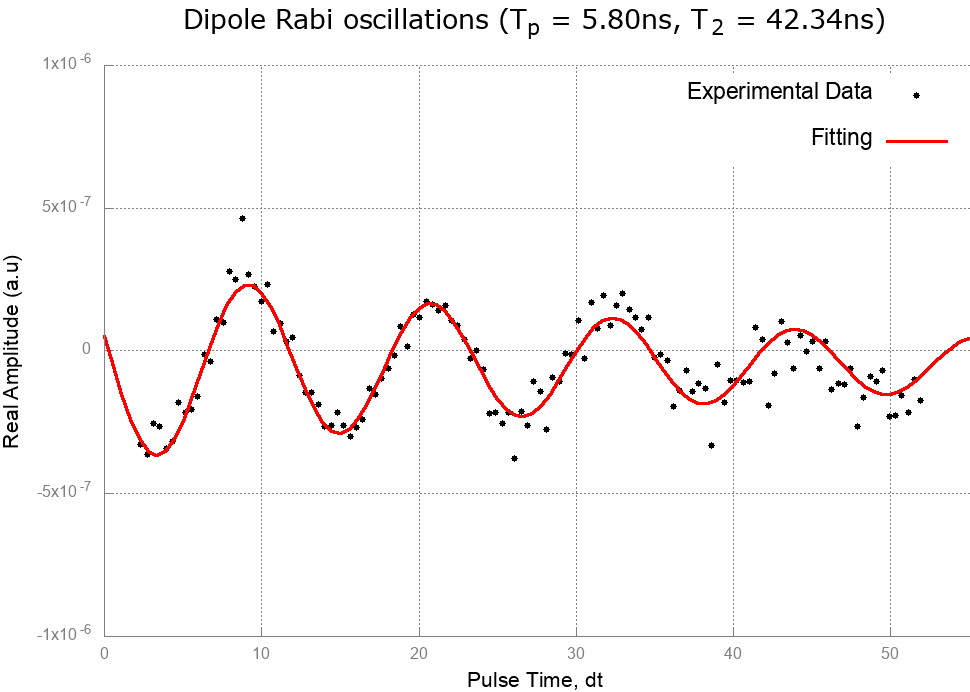
\includegraphics[height = 5cm]{figure5}
   \caption{Rabi oscillation measurements at the degeneracy flux bias, $ \Phi_0/2 $, are made by driving the qubit with resonant
     microwave pulses for different time periods, $ dt $, and monitoring the signal in the output line. The a decoherence time of
     $ T_\varphi = \iunit{42}{ns} $ is extracted from the decay envelope, $ e^{-dt/\tau_\varphi} $, of the the oscillations. \label{fig:rabi}}
 \end{figure}

 \noindent At the degeneracy flux bias $ \sim \varphi_{\text{ext}}(2n+1), n \in \mathbb{Z} $, the energy levels posses a low curvature of
 $ -550\pm10\,\text{GHz}/\Phi_0^2 $ compared with $ 13\times 10^4 \text{GHz}/\Phi_0^2$ \cite{stern2014}, $ 8.4 \times 10^4 \text{GHz}/\Phi_0^2$ \cite{zhu2010} and $ 37\times 10^{4} \text{GHz}/\Phi_0^2$ \cite{gustavsson2012} demonstrated recently on other architectures. Such a broad energy level plateau makes the qubit more robust to flux noise at the operational point. A decoherence time of
 $ \tau_\phi = \iunit{42}{ns} $ is extracted from Rabi oscillations, Fig.~\ref{fig:rabi}, which is high for a qubit fabricated using
 standard nanofabrication technology, without the technological advancements discussed above.
